\documentclass{article}

\usepackage[utf8]{inputenc}
\usepackage{scrextend}
\usepackage[htt]{hyphenat}
\usepackage{graphicx}
\usepackage[edges]{forest}

\definecolor{foldercolor}{RGB}{124,166,198}

\tikzset{pics/folder/.style={code={%
    \node[inner sep=0pt, minimum size=#1](-foldericon){};
    \node[folder style, inner sep=0pt, minimum width=0.3*#1, minimum height=0.3*#1, above right, xshift=0.05*#1] at (-foldericon.west){};
    \node[folder style, inner sep=0pt, minimum size=#1] at (-foldericon.center){};}
    },
    pics/folder/.default={20pt},
    folder style/.style={draw=foldercolor!80!black,top color=foldercolor!40,bottom color=foldercolor}
}

\forestset{is file/.style={edge path'/.expanded={%
        ([xshift=\forestregister{folder indent}]!u.parent anchor) |- (.child anchor)},
        inner sep=1pt},
    this folder size/.style={edge path'/.expanded={%
        ([xshift=\forestregister{folder indent}]!u.parent anchor) |- (.child anchor) pic[solid]{folder=0.7*#1}}, inner sep=0.2*#1},
    folder tree indent/.style={before computing xy={l=0.6*#1}},
    folder icons/.style={folder, this folder size=#1, folder tree indent=3*#1},
    folder icons/.default={12pt},
}
% Margins
\topmargin=-0.45in
\evensidemargin=0in
\oddsidemargin=0in
\textwidth=6.5in
\textheight=9.0in
\headsep=0.25in
\graphicspath{ {./} }

\title{Progetto di Automated Reasoning\\2021-2022}

\author{ Christian Londero }
\date{15 Febbraio 2022}

\begin{document}
\maketitle

\section{Definizione del problema}
Si consideri una scacchiera $n$ x $n$ ($n$ è dato in input). Si hanno a disposizione $l$ pezzi a forma di L, $s$ pezzi a forma di quadrato e $r$ pezzi a forma di rettangolo (si veda la figura, la dimensione del rettangolo è 3 x 1, il quadrato è 2 x 2 e il lato lungo della L è 2). $l$, $s$, $r$ sono dati in input. L'obbiettivo è di riempire la scacchiera con i pezzi a disposizione in maniera tale da minimizzare le celle vuote/free. Il requisito aggiuntivo è che $f$ celle (date in input) siano già occupate (quindi vietate).\\
Si veda l'esempio (le celle grigie sono già occupate/vietate).

\subsection{Considerazioni}
Si presenterà un algoritmo che tenta di minimizzare le celle empty scegliendo da un sottoinsieme dei pezzi. \\
Quindi si può dare in input un numero molto alto di pezzi al fine di ``semplificare" la minimizzazione, sebbene si rischia in questo caso di fare utilizzare gli stessi tipi di pezzi quasi ovunque.\\
Nella sezione dei risultati vedremo infatti che se abbiamo a disposizione un elevato numero di pezzi ($3*l + 4*s + 3*r \gg n*n$) allora il solving è ``facile", rispetto a un numero quasi giusto di pezzi ($3*l + 4*s + 3*r \simeq n*n$).

\section{Soluzione}
L'idea utilizzata per la realizzazione dei modelli è la stessa sia per il modello in minizinc che per quello in asp. Parlando a livello non-implementativo, è la seguente: il programma prende in input i seguenti parametri:
\begin{itemize}
    \item \texttt{n} (intero): dimensione della board;
    \item \texttt{l} (intero): numero di L (2x2) disponibili;
    \item \texttt{s} (intero): numero di quadrati (2x2) disponibili;
    \item \texttt{r} (intero): numero di rettangoli (1x3) disponibili;
    \item \texttt{f} (intero): numero di celle vietate/forbidden/già occupate;
    \item \texttt{forbidden} (array): array lungo $f$ di coordinate $X,Y$ (sono dei fatti/facts in asp).
\end{itemize}
La board è una matrice (array bi-dimensionale) $n$ x $n$ il cui dominio è definito dalla seguente enumerazione: \texttt{XXX, EEE, S11, S12, S13, S14, R11, R12, R13, R21, R22, R23, L11, L12, L13, L21, L22, L23, L31, L32, L33, L41, L42, L43}.\\
Al fine di rendere comprensibile l'enumerazione si osservi la figura qui di seguito.\\
\begin{figure}[ht!]
    \centering
    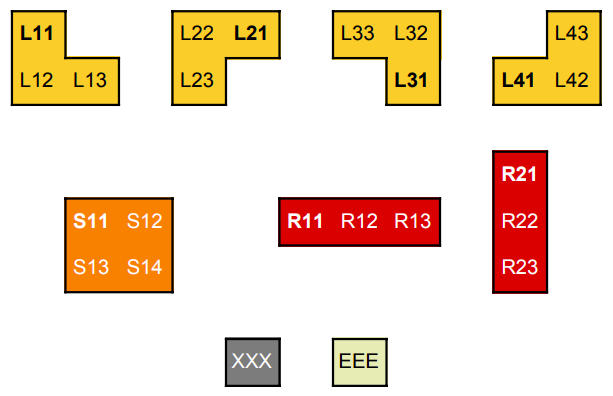
\includegraphics[width=0.7\textwidth]{images/shapes}
    \caption{Tutte le possibili shapes con rotazioni}
\end{figure}
Quindi ogni cella può assumere uno di quei valori dell'enumerazione, si è quindi proceduto a definire dei vincoli che mantengano le forme corrette.\\
Ho utilizzato tale ``metodo" al fine di evitare sovrapposizioni indesiderate dei pezzi. \\
E' possibile visualizzare il modello di minizinc a \texttt{./main.mzn} e di clingo/ASP a \texttt{./main.lp} per ulteriori dettagli implementativi.\\
Per minizinc non sono state definite delle annotazioni di ricerca particolari (sebbene siano state tentate ma con migliorie pressochè nulle).\\\\
ASP/clingo viene lanciato con i seguenti parametri:\\\\
\hspace*{.5cm}\texttt{clingo $main.lp$ $input$ -t8 --quiet=1,1 --out-hide-aux --outf=2 --time-limit=300 --warn none --configuration=frumpy --opt-strategy=bb,inc}\\\\
di cui gli unici di ottimizzazione \texttt{-t8 --configuration=frumpy --opt-strategy=bb,inc}; si è infatti evidenziato un notevole miglioramento dei tempi di risoluzione per certe istanze mediante l'ausilio di tali parametri. I restanti parametri sono utili solo a formattare l'output in un modo agevole per essere parsato dal \texttt{visualizer} (di cui discuteremo nella sezione 4).\\
Minizinc viene lanciato con i seguenti parametri:\\\\
\hspace*{.5cm}\texttt{minizinc $main.mzn$ $input$ -O2 --solver {} --time-limit 300000 -p12 -f --output-mode json -s --soln-separator ``" --search-complete-msg ``OPTIMUM"}\\\\
di cui gli unici di ottimizzazione sono \texttt{--O2 -f}. Il primo risulta il miglior compromesso tra tempo di compilazione e guadagno in termini di tempi nella fase di risoluzion; il secondo invece, \texttt{-f} (free search), migliora i tempi di molte istanze prese in analisi. I restanti parametri sono utili solo a formattare l'output in modo agevole per il \texttt{visualizer}.

\subsection{Ulteriori idee}
Avevo pensato ad altre due modellazioni che però nell'implementazione poi si sono rivelate errate/inefficienti:
\begin{itemize}
    \item indicare con 1 le L, con 2 i quadrati e con 3 i rettangoli, con 0 le empty cells e con -1 i forbidden; tuttavia, sebbene il dominio in questo casi sia notevolmente ridotto, con tale metodo non si riescono a gestire efficientemente le sovrapposizioni di forme uguali con diverse rotazioni
    \item enumerare ogni pezzo mantenendo il tipo salvato in un ``array" lungo $k$ con $k=l+s+r$ (per esempio, ignorando le celle empty e forbidden, se abbiamo $k=2+1+3$ avremmo che il dominio delle celle della board è $1..k$ = $1..6$ e manteniamo un ulteriore array lungo k per indicare il tipo: [1,1,2,3,3,3]), in modo tale che il tipo indichi quali constraint il pezzo i-esimo debba avere e non ci sono sicuramente sovrapposizioni in quanto un pezzo di forma uguale avrebbe un $j!=i$ come ``valore" e ogni ``valore" può comparire al più 3 o 4 volte nella board a seconda della forma (rispettivamente se L/rettangolo o quadrato); tuttavia questo metodo si è rivelato altamente inefficiente in quanto i domini erano molto più grandi rispetto alla soluzione scelta e portavano quindi a tempi molto più elevati anche con strategie di \texttt{int\_search} (per minizinc) personalizzate;
\end{itemize}

\section{Utilities}
Sono state predisposte alcune utilities per velocizzare la fase di test. In particolare nella folder \texttt{./utils/} si trovano:
\begin{itemize}
    \item \texttt{input\_gen.py} che prende in input 7 parametri:
          \begin{enumerate}
              \item $q$: il numero di istanze (diverse) che vogliamo generare;
              \item $n$: dimensione della board;
              \item $l$: numero di L 2x2;
              \item $s$: numero di quadrati 2x2;
              \item $r$: numero di rettangoli 1x3;
              \item $f$: numero di celle proibite (scelte random);
              \item $output\_path$ (OPZIONALE): path alla cartella dove verranno inseriti gli input generati; qualora non specificato, crea gli input salvandoli nella folder \texttt{../inputs} (che viene creata in automatico).
          \end{enumerate}
          Genera sia il \texttt{dzn} che il \texttt{lp}. Un esempio di esecuzione:
          \texttt{python utils/input\_gen.py 1 10 10 7 10 10 10} 
    \item \texttt{run\_tests.py} che prende in input 2 parametri:
          \begin{enumerate}
              \item $input\_path$ (OPZIONALE): path alla cartella dove verranno cercati gli input da lanciare; qualora non specificato, cerca gli input nella folder \texttt{../inputs};
              \item $output\_path$ (OPZIONALE): path alla cartella dove verranno inseriti gli output generati; qualora non specificato, crea gli output salvandoli nella folder \texttt{../outputs} (che viene creata in automatico).
          \end{enumerate}
          esegue i rispettivi visualizer a seconda del tipo di file in input. Genera anche un file \texttt{metadata.csv} all'interno dell'$output\_path$ che contiene le info circa l'esecuzione di ciascun solver (qualora non ci fossero errori). Un esempio di esecuzione:\\
          \texttt{python utils/run\_tests.py}
\end{itemize}

\section{Visualizer delle soluzioni}
Per agevolare la visualizzazione dell'output dei solver (sia asp che minizinc) è stato predisposto un \texttt{visualizer}, splittato per clingo e minizinc, scritto in python che riceve in input il main, l'input e opzionalmente dove salvare l'output e restituisce un file html che renderizza la griglia trovata dal solver (se non restituisce errori) in formato HTML + CSS.\\
Più tecnicamente, per stampare l'output dell'input $i$ di clingo/asp salvato nella folder ./inputs/input$i$.lp (o di minizinc salvato nella folder ./inputs/input$i$.dzn), si può lanciare il seguente comando:\\\\
\hspace*{.5cm}\texttt{python visualizer/asp\_visualize.py main.lp inputs/input$i$.lp outputs/asp$i$.html}\\
\hspace*{.5cm}\texttt{python visualizer/mzn\_visualize.py $solver$ main.mzn inputs/input$i$.dzn outputs/mzn-$solver$$i$.html}\\\\
e aprendo il file \texttt{outputs/asp$i$.html} (o mzn-$solver$$i$.html) si potrà visualizzare la soluzione visivamente con le relative stats. Per minizinc $solver$ può essere $gecode$ oppure $coinbc$.\\
Sia minizinc che ASP all'interno dei rispettivi visualizer vengono eseguiti con dei parametri customizzati per restituire gli output in json per poi essere utilizzati comodamente dal visualizer. I parametri di ottimizzazione invece vengono descritti nella sezione successiva.\\
Il terzo parametro è opzionale. Qualora non fosse specificato, l'output viene salvato automaticamente nella folder \texttt{outputs}.\\
I colori dei pezzi sono:
\begin{itemize}
    \item L: giallo
    \item quadrato: arancione
    \item rettangolo: rosso
    \item empty cell: bianca
    \item forbidden cell: grigia
\end{itemize}
\begin{figure}[ht!]
    \centering
    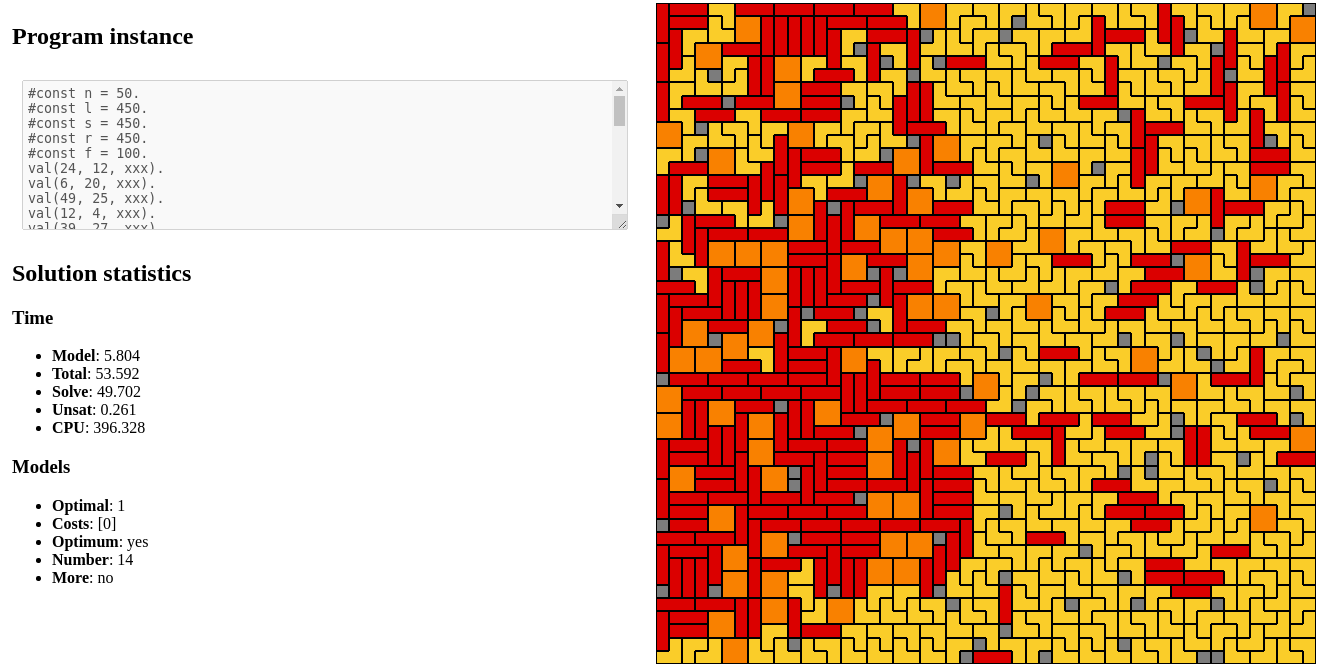
\includegraphics[width=0.7\textwidth]{images/visualizer.png}
    \caption{Esempio del visualizer sull'input 12 di ASP/clingo}
\end{figure}


\section{Risultati sperimentali}
I test sono stati effettuati su un PC con OS Ubuntu 18.04, con 8GB di RAM e CPU intel core i7 4770HQ@2.20GHz.\\
Il modello di ASP risulta molto più performante rispetto a quello di minizinc per la maggior parte degli input analizzati. La suddivisione in istanze easy/medium/hard verrà fatta in base al tempo minore di risoluzione tra minizinc e ASP.\\
Per minizinc sono stati studiati i comportamenti dei solver gecode e coinbc. Il solver coinbc risultava particolarmente più efficace rispetto a gecode per il modello definito. \\Si noti che il modello di minizinc restituisce un ``out of memory" da $n=50$ in poi, sebbene comunque risulti ``affaticato" già con istanze aventi un $n$ minore.\\
D'altrocanto il modello ASP fatica a ``confermare" l'ottimo trovato con istanze aventi (un numero di) pezzi ``quasi giusti" che riescono a ricoprire l'area copribile ($n*n - f$), si veda infatti l'input numero 4. Il problema invece non si pone per istanze aventi un numero di pezzi insufficienti a coprire l'intera area copribile, in quanto è stato definito un lower bound al ``minimo" di celle empty (\texttt{main.lp:40}).\\\\
E' possibile visualizzare ogni input/output dei risultati proposti di seguito (come output dei rispettivi \texttt{visualizer}) nella cartella \texttt{./examples/outputs}. Per ogni output c'è il prefisso relativo al solver/metodo utilizzato (asp, minizinc-gecode, minizinc-coinbc). Qualora non fosse disponibile un output, il motivo è che il solver è andato in out of memory.\\I costi vengono evidenziati in grassetto qualora l'output sia un ottimo.

\subsection{Istanze ``easy"}
Per istanza easy del problema (relativa alla soluzione proposta) si intende o un problema con $n$ relativamente piccolo, oppure un problema con $n$ non molto grande ma avendo a disposizione $k$ pezzi con $area(k) \gg n*n-f$ (quindi l'area di tutti i pezzi disponibili ``eccessivamente" maggiore rispetto all'area copribile). Di seguito una tabella che riassume alcuni casi ``easy" con $f$ celle scelte a random.\\

\begin{figure}[ht!]
    \centering
    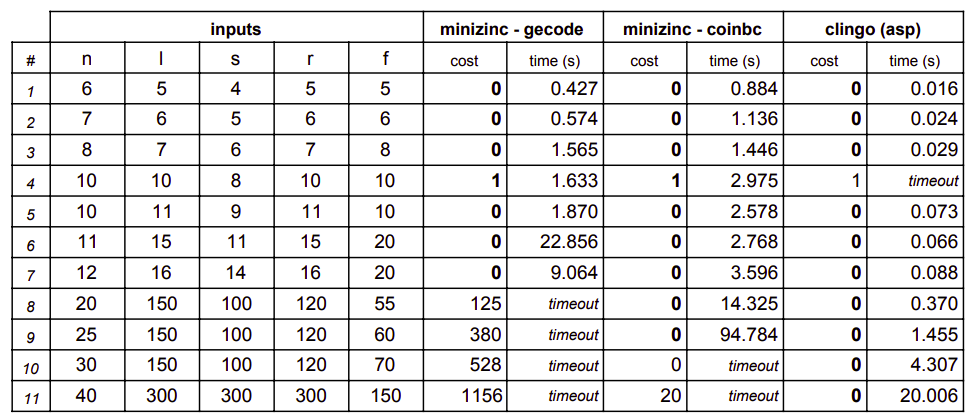
\includegraphics[width=0.7\textwidth]{images/easy-instances.png}
    \caption{Easy instances}
\end{figure}

\subsection{Istanze ``medium"}
Per istanza media del problema (relativa alla soluzione proposta) si intende un problema con $n$ relativamente grande (tra 50 e 60)  avendo a disposizione $k$ pezzi con $area(k) \gg n*n-f$ (quindi l'area di tutti i pezzi disponibili ``eccessivamente" maggiore rispetto all'area copribile). Di seguito una tabella che riassume alcuni casi ``medium" con $f$ celle scelte a random.\\

\begin{figure}[ht!]
    \centering
    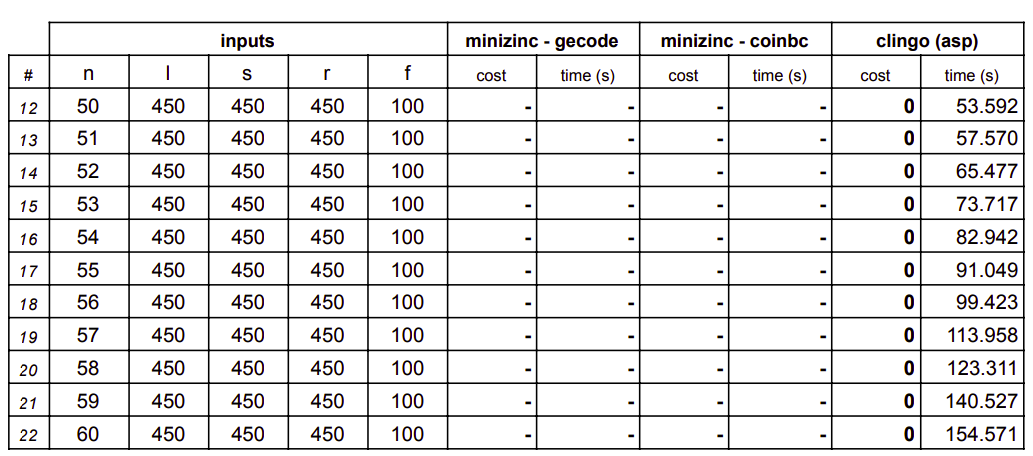
\includegraphics[width=0.7\textwidth]{images/medium-instances.png}
    \caption{Medium instances}
\end{figure}

\subsection{Istanze ``hard"}
Per istanza hard del problema (relativa alla soluzione proposta) si intende o un problema con $n$ grande ($n > 60$) con (un numero di) pezzi ``quasi giusti" che riescono a ricoprire l'area copribile ($n*n - f$) oppure un problema con $n > 70$. Di seguito una tabella che riassume alcuni casi ``hard" con $f$ celle scelte a random.\\

\begin{figure}[ht!]
    \centering
    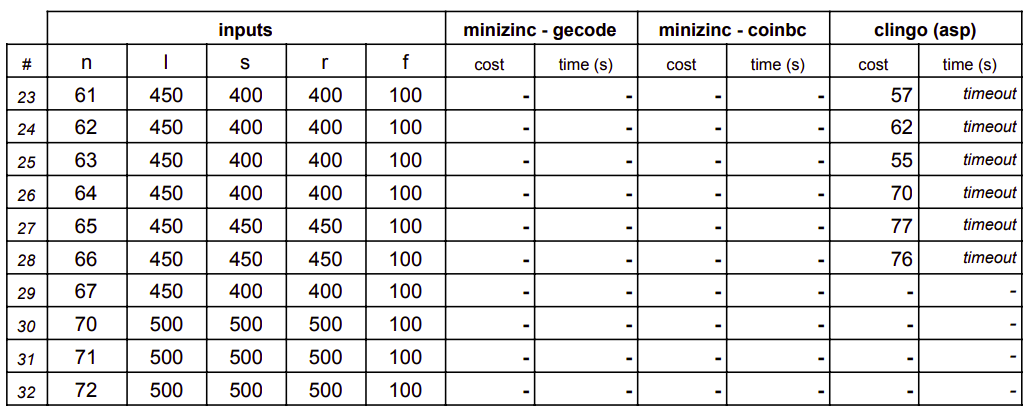
\includegraphics[width=0.7\textwidth]{images/hard-instances.png}
    \caption{Hard instances}
\end{figure}

\end{document}